\documentclass[a4paper, 12pt]{article}
\usepackage[utf8]{inputenc}
\usepackage{geometry}
\usepackage{polski}
\usepackage{graphicx}
\usepackage{float}
\usepackage{etoolbox,refcount}
\usepackage{multicol}
\usepackage{tabularx}

\newgeometry{left=2cm, right=2cm, bottom=2cm, top=1.5cm}

\begin{document}
	\begin{figure}[H]
		\centering
		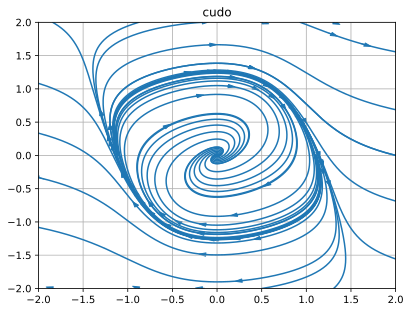
\includegraphics[width = \textwidth]{./img/cudo.png}
	\end{figure}
	\section{Cel ćwiczenia}
		Celem ćwiczenia jest zapoznanie się z metodami doboru nastaw regulatora przemysłowego metodą Zieglera--Nicholsa (łącznie z modyfikacjami) oraz przy pomocy metod opartych o parametry odpowiedzi skokowej obiektu.
	\section{Wstęp}
		\subsection{Schemat w SIMULINKu}
			Poniższy schemat przedstawia zastosowane przez nas połączenie bloczków w SIMULINKu. Połączenia zostały dokonane zgodnie z instrukcją, dodatkowo dodaliśmy do nich wyprowadzenie na ekran przedstawiający całkę z kwadratu uchybu.
			\begin{figure}[H]
				\centering
				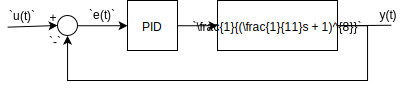
\includegraphics[width = \textwidth]{./img/schemat.png}
			\end{figure}
		\subsection{Wstępne obliczenia}
			Postanowiliśmy przed wykonywaniem ćwiczenia dokonać wstępnych obliczeń, które pozwolą nam sprawdzić, czy dobrze wyznaczyliśmy wzmocnienie krytyczne. Postanowiliśmy wyznaczyć je z kryterium Nyquista, posługując się do tego prostym skryptem rysującym charakterystykę Nyquista dla obiektu w układzie otwartym. Skrypt następnie powiększa interesujący nas fragment charakterystyki i wymaga od użytkownika aby ten jak najdokładniej (najlepiej wielokrotnie) zaznaczył najbliższy punkowi (-1, 0) punkt przecięcia charakterystyki z osią rzeczywistą. Wzmocnienie krytyczne jest następnie obliczane na podstawie zależności $K_{kr} = -\frac{1}{x}$, gdzie jako x jest brana średnia arytmetyczna z części rzeczywistej zaznaczonych punktów.
			\begin{figure}[H]
				\includegraphics[width = \textwidth]{./code/teoria.png}
			\end{figure}
			\noindent
		\subsection{Przebieg dla wzmocnienia krytycznego}
			Poniższy przebieg przedstawia symulację dla wyliczonego tym sposobem $K_{kr} = 5,3685$. Mamy tu do czynienia z oscylacjami nietłumionymi -- wynika z tego, że wyznaczona wartość jest poprawna.
			\begin{figure}[H]
				\centering
				\includegraphics[width = \textwidth]{./img/teoretyczne.png}
			\end{figure}
	\section{Wyniki}
		Po wstępnych obliczeniach przystąpiliśmy do wyznaczenia krytycznej wartości wzmocnienia metodą opisaną w ćwiczeniu. Jednak aby przyśpieszyć całość postanowiliśmy napisać do tego skrypt:
		\begin{figure}[H]
			\includegraphics[width = \textwidth]{./code/desperate.png}
		\end{figure}
		\noindent
		Wyniki dla niektórych wartości sprawdzanego wzmocnienia:
		\begin{figure}[H]
			\centering
			\includegraphics[width=0.48\linewidth]{./img/szukanie_k_1.png}
			\includegraphics[width=0.48\linewidth]{./img/szukanie_k_5.png}
			\includegraphics[width=0.48\linewidth]{./img/szukanie_k_5_3.png}
			\includegraphics[width=0.48\linewidth]{./img/szukanie_k_5_4.png}
			\includegraphics[width=0.48\linewidth]{./img/szukanie_k_5_5.png}
			\includegraphics[width=0.48\linewidth]{./img/szukanie_k_7.png}
		\end{figure}
		\noindent
		Na podstawie tych przebiegów można odczytać, że najbliższą wartości wzmocnienia krytycznego jest wzmocnienie $K_p = 5,4$, gdyż wtedy przebieg najbardziej przypomina oscylacje nierozbiegające się i nietłumione. Jest to zgodne z uprzednio wykonanymi obliczeniami.
		\newline
		\newline 
		Ponieważ bloczek PID w SIMULINKu wymaga danych podanych w formie PID IND oraz ponieważ chcieliśmy zautomatyzować wyznaczanie chwili w której uchyb spadnie poniżej 1\% swojej wartości początkowej postanowiliśmy napisać dwie funkcje. Jedna przyjmuje jako argumenty parametry bloczka PID ISA i zwraca nastawy bloczka PID IND, a druga przyjmuje za argumenty współrzędne x oraz y punktów przebiegów i zwraca chwilę czasu od której przebieg mieści się w przedziale wartości [0,99 , 1,01] i w nim pozostaje.
		\begin{figure}[H]
			\includegraphics[width = \textwidth]{./code/get_IND.png}
		\end{figure}
		\noindent
		Powyższy kod dla zerowego czasu zdwojenia wyłącza akcję całkującą.
		\begin{figure}[H]
			\includegraphics[width = \textwidth]{./code/time_until_stable.png}
		\end{figure}
		\noindent
		Powyższy kod w chwili wejścia do przedziału zaczyna pętlę, która iteruje tak długo aż wyjdziemy z zadanego przedziału wartości albo aż skończą się nam argumenty wejściowe. Przed wejściem do pętli zapamiętuje czas dla jakiego się to dokonało. 
		\newline 
		\newline
		Wartość przeregulowania oraz czas potrzebny do osiągnięcia przez układ uchybu poniżej 1\% wartości początkowej są sensowne tylko dla przypadków, gdzie mamy do czynienia z zerowym uchybem ustalonym oraz przeregulowaniami.
		\newpage
		\noindent
		\subsection{Regulator P - metoda Zieglera-Nicholsa}
			Na przebiegu można zauważyć wystąpienie uchybu ustalonego -- bierze się to z braku akcji całkującej w regulatorze, uniemożliwia to wyznaczenie czasu po którym układ dochodzi do stanu gdy uchyb ma wartość 1\% wartości początkowej. Układ posiada małe przeregulowanie, a z powodu uchybu ustalonego całkowy wskaźnik jakości pozbawiony jest sensu -- całka jest niezbieżna, a przybliżenie słabe.
			\begin{figure}[H]
				\centering
				\includegraphics[width = 0.7\textwidth]{./img/ZN_P.png}
			\end{figure}
		\subsection{Regulator PI - metoda Zieglera-Nicholsa}
			Ze względu na występowanie akcji całkującej w regulatorze występuje zerowy uchyb ustalony. Całka z kwadratu uchybu jest zbieżna i wystarczające jest policzenie jej w przedziale czasowym od początku do końca symulacji. Przeregulowanie jest niższe niż w przypadku regulatora P.
			\begin{figure}[H]
				\centering
				\includegraphics[width = 0.7\textwidth]{./img/ZN_PI.png}
			\end{figure}
		\subsection{Regulator PD - metoda Zieglera-Nicholsa}
			Podobnie jak regulator typu P regulator PD posiada uchyb ustalony, co wyklucza go z rozważań w kategorii całkowego współczynnika jakości regulacji. Przeregulowania występujące tu są znaczne w porównaniu do dwóch poprzednich przypadków, a układ znacznie gorzej znosi opóźnienia powodując bardzo powolne tłumienie oscylacji.
			\begin{figure}[H]
				\centering
				\includegraphics[width = 0.7\textwidth]{./img/ZN_PD.png}
			\end{figure}
		\subsection{Regulator PID - metoda Zieglera-Nicholsa}
			W przebiegu nie jesteśmy w stanie zaobserwować przeregulowania. Układ źle znosi opóźnienia ze względu na część różniczkującą, która powoduje, że przebieg jest poszarpany. Przebieg stabilizuje się nieznacznie szybciej niż w przypadku regulatora PI oraz posiada lepszy współczynnik jakości regulacji.
			\begin{figure}[H]
				\centering
				\includegraphics[width = 0.7\textwidth]{./img/ZN_PID.png}
			\end{figure}
		\subsection{Regulator PID z niewielkimi przeregulowaniami - metoda Zieglera-Nicholsa}	
			Ze względu na strasznie poszarpany kształt przebiegu odpowiedzi układu nie jesteśmy w stanie wyznaczyć przeregulowań. Czas potrzebny do stabilizacji jest znacznie dłuższy niż w pozostałych regulatorach. Współczynnik jakości regulacji jest prawie tak samo dobry jak w przypadku regulatora PID oraz lepszy niż w przypadku regulatora PI.
			\begin{figure}[H]
				\centering
				\includegraphics[width = 0.7\textwidth]{./img/ZN_PID_small.png}
			\end{figure}
		\subsection{Regulator PID bez przeregulowań - metoda Zieglera-Nicholsa}
			Można zaobserwować tu brak przeregulowań. Współczynnik jakości regulacji jest porównywalny do regulatora PI, jednak czas potrzebny do wytłumienia oscylacji jest znacznie większy niż\linebreak w przypadku poprzednich regulatorów. Maksymalna wartość przebiegu jest najmniejsza spośród układów posiadających zerowy uchyb ustalony.
			\begin{figure}[H]
				\centering
				\includegraphics[width = 0.7\textwidth]{./img/ZN_PID_no.png}
			\end{figure}
		\subsection{Passen integral rule}
			Te nastawy regulatora pozwalają na zaobserwowanie dużego przeregulowania. Skrajne wartości przebiegu są nieakceptowalne w wielu procesach technologicznych ze względu na swoją zmienność oraz nagłe zmiany sterowania regulatora. Współczynnik jakości jest lepszy niż dla regulatora PI, jednak gorszy niż w przypadku regulatora PID. Duży czas potrzebny do stabilizacji wyklucza te nastawy regulatora z wielu zastosowań.
			\begin{figure}[H]
				\centering
				\includegraphics[width = 0.7\textwidth]{./img/passen.png}
			\end{figure}
		\subsection{Tyreus-Luyben - PI}
			Regulator ten nie posiada przeregulowań. Wartości utrzymują się ciągle poniżej wartości zadanej, co pozwala na zastosowanie tego regulatora w przypadkach, gdzie dana wartość nie może być przekroczona -- np. podgrzewanie łatwopalnych chemikaliów. Wadą tego rozwiązania jest kiepski współczynnik jakości regulacji oraz kiepski czas regulacji.
			\begin{figure}[H]
				\centering
				\includegraphics[width = 0.7\textwidth]{./img/Tyr-Luy_PI.png}
			\end{figure}
		\subsection{Tyreus-Luyben - PID}
			W porównaniu do poprzedniego regulatora ma on niewiele krótszy czas regulacji oraz lepszy współczynnik jakości sterowania. Podobnie jak on może być używany w przypadkach kiedy nie możne zostać przekroczona pewna wartość, jednak z uwagą na możliwość zniszczenia elementów wykonawczych ze względu na występujące pojedyncze gwałtowne zmiany sygnału wyjściowego.
			\begin{figure}[H]
				\centering
				\includegraphics[width = 0.8\textwidth]{./img/Tyr-Luy_PID.png}
			\end{figure}				
	\section{Wnioski}
		Ćwiczenie te pozwoliło nam na zapoznanie się z dobieraniem nastaw regulatorów metodą Zieglera--Nicholsa oraz pozwoliło nam na porównanie całkowego współczynnika jakości $\int_0^\infty e^2(t) \mathrm{d}t$ regulatora z nastawami według metody Zieglera--Nicholsa z innymi nastawami. Zgodnie z przewidywaniami teoretycznymi jest on lepszy dla nastaw z metody Zieglera--Nicholsa niż dla pozostałych nastaw.
		\newline
		\newline
		Zobaczyliśmy negatywny wpływ opóźnienia na regulację procesu. W połączeniu z członem różniczkującym opóźnienie powoduje gwałtowne zmiany sygnału, które potencjalnie mogłyby uszkodzić resztę układu. 
		\newline
		\newline
		Dowiedzieliśmy się o innych metodach doboru nastaw oraz o ich wadach i zaletach. Wiemy gdzie możemy używać pewne nastawy oraz gdzie stanowią pewne niebezpieczeństwo oraz gdzie muszą zastąpić regulatory PID z nastawami dobranymi metodą Zieglera--Nicholsa.
\end{document}